\documentclass{beamer}
\usepackage[utf8]{inputenc}
\usepackage[T1]{fontenc}
\usepackage[french]{babel}
\usepackage{graphicx}
\usepackage{hyperref}

\title{Prospection Système Solaire}
\subtitle{Document de Présentation}
\author{Astraea Mining Corp}
\date{2150}

\begin{document}

\begin{frame}
    \titlepage
\end{frame}

\begin{frame}
    \frametitle{Concept du Jeu}
    \begin{itemize}
        \item \textbf{Prospection Système Solaire} est un jeu de simulation spatiale se déroulant en l'an 2150.
        \item Incarnez un prospecteur indépendant travaillant pour Astraea Mining Corp.
        \item Explorez le système solaire avec ses orbites planétaires dynamiques.
        \item Collectez des ressources, améliorez votre équipement et gérez votre réputation auprès des différentes factions (Coalition Terrestre, République Martienne, Alliance de la Ceinture, Consortium Jovien).
    \end{itemize}
\end{frame}

\begin{frame}
    \frametitle{Votre Vaisseau: Astraea-I}
    \begin{center}
        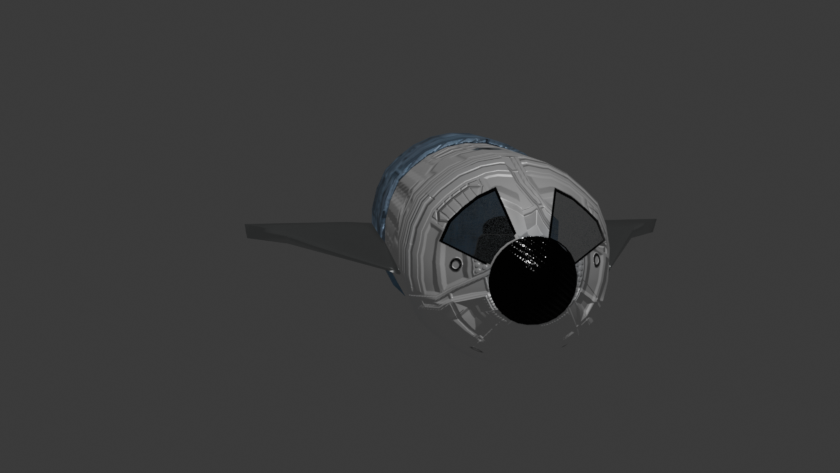
\includegraphics[height=0.6\textheight]{ship.png}
    \end{center}
    \begin{itemize}
        \item Navette de Prospection Légère.
        \item Équipée de lasers de minage, de scanners et d'une soute modulable.
        \item Amélioration possible des moteurs, boucliers et systèmes d'extraction.
    \end{itemize}
\end{frame}

\begin{frame}
    \frametitle{Station Orbitale}
    \begin{center}
        \includegraphics[width=0.8\textwidth]{station.png}
    \end{center}
\end{frame}

\begin{frame}
    \frametitle{Équipement du Pilote}
    \begin{center}
        \includegraphics[height=0.6\textheight]{suit.png}
    \end{center}
    \begin{itemize}
        \item Combinaison de vol haute technologie pour les environnements hostiles.
    \end{itemize}
\end{frame}

\begin{frame}
    \frametitle{Aperçu en Jeu}
    \begin{center}
        \includegraphics[width=0.9\textwidth]{gameplay1.png}
    \end{center}
\end{frame}

\end{document}
